%-------------------------------------------------------------------------
\section{Evaluation}
\label{sec:evaluation}

We conducted four different evaluations on PARSEWeb to show that
PARSEWeb is effective in solving programmers' queries. In the
first evaluation, we showed that PARSEWeb is able to solve
programming problems posted in developer forums of existing
libraries. In the second evaluation, we showed that
PARSEWeb-suggested solutions are available in \realprojects{}. We
also analyzed the PARSEWeb results with the results of two other
related tools:
Prospector\footnote{\url{http://snobol.cs.berkeley.edu/prospector/}}~\cite{prospector:jungloid}
and
Strathcona\footnote{\url{http://strathcona.cpsc.ucalgary.ca/}}~\cite{strathcona:se}.
Prospector tries to solve the queries related to a specific set of
frameworks or libraries by using API signatures. Strathcona tries to
suggest similar code examples stored in an example repository by
matching the context of the code under development with the samples
stored in the example repository. In the third evaluation, we
compared PARSEWeb with Prospector. We showed that PARSEWeb performs
better than Prospector. Moreover, PARSEWeb is not limited to the
queries of any specific set of frameworks or libraries as Prospector
is. In the fourth evaluation, we showed the significance of different techniques used
in PARSEWeb.

%-------------------------------------------------------------------------
\subsection{Programming Problems}
\label{sec:subexperiments}

The purpose of this evaluation is to show that PARSEWeb is not
limited to the queries of any specific set of frameworks or
libraries. We collected two programming problems that were posted
by developers in forums of existing open source frameworks or
libraries and checked whether PARSEWeb is able to suggest solutions
for those problems; existing tools such as Prospector and Strathcona
cannot address these problems because the queries for these problems
fall out of the scope of these two tools: J2SE, Eclipse, and Eclipse
GEF (Graphical Editing Framework). The results indicate that PARSEWeb is able to solve
these real programming problems.

%-------------------------------------------------------------------------
\subsubsection{Jakarta BCEL User Forum}

The Byte Code Engineering Library (BCEL) provides the ability to
analyze, create, and manipulate Java bytecode files.\Comment{BCEL is
already being used successfully in several projects such as
compilers, optimizers, and code generators.} We collected the
programming problem ``How to disassemble Java byte code'' posted in
the BCEL forum~\cite{BCELForum}. The programming problem describes
that the programmer is using the BCEL library and has Java byte code
under analysis. In the BCEL library, Java byte code is represented
through the \CodeIn{Code} class. The programmer wants to obtain a
Java assembler command list, which is represented in the form of
instructions in the BCEL library. Therefore, we identified the
relevant query for the given problem description as ``\CodeIn{Code}
$\rightarrow$ \CodeIn{Instruction}''. PARSEWeb suggested a solution
for the query as shown below:

\begin{CodeOut}
\begin{alltt}
01:FileName:2\_RepMIStubGenerator.java MethodName:
\hspace*{0.2in}isWriteMethod Rank:1 NumberOfOccurrences:1
02:Code,getCode() ReturnType:\#UNKNOWN\#
03:CONSTRUCTOR,InstructionList(\#UNKNOWN\#)
\hspace*{0.2in}ReturnType:InstructionList
04:InstructionList,getInstructions() 
\hspace*{0.2in}ReturnType:Instruction
\end{alltt}
\end{CodeOut}

The suggested solution is the same as the response posted in the forum. The programmer
can refer to a related code sample by browsing the \CodeIn{isWriteMethod} method
in the file \CodeIn{2\_RepMIStubGenerator.java}. 
The original code sample collected from the
preceding method is shown below:

\begin{CodeOut}
\begin{alltt}
Code code;
InstructionList il = new InstructionList(code.getCode());
Instruction[] ins = il.getInstructions();
\end{alltt}
\end{CodeOut}

In the code sample suggested by PARSEWeb, the return type of
\CodeIn{getCode} method is described as \CodeIn{UNKNOWN}. The keyword
\CodeIn{UNKNOWN} denotes that the PARSEWeb is not able to infer the
return type through its heuristics, because the return type of
\CodeIn{getCode} method is not explicitly specified in the code
sample. However, PARSEWeb still correctly suggested to pass the
return type directly to the constructor of \CodeIn{InstructionList}.
%-------------------------------------------------------------------------

\Comment{\subsubsection{Java Media Framework forum}

The Java Media Framework API (JMF) enables audio, video, and other
time-based media to be added to applications and applets built on
Java technology. We collected the programming problem ``Get the Data
from a DataSource'' posted by a JMF developer from the JMF
forum~\cite{JMFForum}. The main objective of the problem was to get
raw data from an object of type \CodeIn{Processor}. We transformed
the problem into the query ``\CodeIn{Processor $\rightarrow$}
\CodeIn{PushBufferStream}'' by using the description given in the
problem. We specified the \emph{Destination} as
\CodeIn{PushBufferStream}, because raw data can be obtained from a
\CodeIn{BufferStream} object. We used PARSEWeb to solve the problem
and posted the solution in the forum to get developers feedback. The
solution suggested by PARSEWeb is shown below.  In the output of
PARSEWeb, the keyword ``DownCasted\_ReturnType'' indicates that an
explicit typecast has to be performed.

\begin{CodeOut}
\begin{alltt}
01: FileName:0\_CamDriver.java MethodName:initImageFetcher
02: \hspace*{0.2in}Rank:1 NumberOfOccurrences:1 Path:1 2
03: \hspace*{0.1in}javax.media.Processor,getDataOutput()
04: \hspace*{0.2in}DownCasted\_ReturnType:
05: \hspace*{0.2in}javax.media.protocol.PushBufferDataSource
06: \hspace*{0.1in}javax.media.protocol.PushBufferDataSource,getStreams()
07: \hspace*{0.2in}ReturnType:javax.media.protocol.PushBufferStream
\end{alltt}
\end{CodeOut}}
%-------------------------------------------------------------------------
\subsubsection{Dev2Dev Newsgroups}

We applied PARSEWeb on another problem ``how to connect db by
sessionBean'' posted in the Dev2Dev Newsgroups~\cite{BEAForum}. We
transformed the question into the query ``\CodeIn{InitialContext
$\rightarrow$ Connection}'' and used PARSEWeb to obtain the
solution. PARSEWeb suggested the following solution, which is the
same as the one described in the forum.

\begin{CodeOut}
\begin{alltt}
01:FileName:3\_AddrBean.java MethodName:getNextUniqueKey
\hspace*{0.2in}Rank:1 NumberOfOccurrences:34
02:InitialContext,lookup(String) ReturnType:DataSource
03:DataSource,getConnection() ReturnType:Connection
\end{alltt}
\end{CodeOut}

%-------------------------------------------------------------------------
\subsection{Real Project}

\Comment{ \setlength{\tabcolsep}{1pt}
\begin{table}[t]
%\begin{alltt}
\begin{CodeOut}
\begin{center}
\centering \caption {\label{table:codesamples} Suggested Code
Samples}
\begin {tabular} {|l|l|}
\hline \textbf{Original Code}&\textbf{PARSEWeb}\\
\hline
public void init(IPageSite &FileName:0\_JDEv...Editor.java \\
\hspace*{0.2in}pageSite)\{...&\hspace*{0.2in}MethodName:init Rank:1 \\
IActionBars bars = &NumberOfOccurrences:7 \\
\hspace*{0.2in}pageSite.getActionBars();&org.eclipse.ui.part.IPageSite\\
&,getActionBars()\\
\}&RetType:org.eclipse.ui.IActionBars\\
\hline \textbf{Prospector}&\textbf{Strathcona}\\
\hline org.eclipse.ui.part.IPageSite ips;&IActionBars actionBars =\\
org.eclipse.ui.IActionBars iab = &pageSite.getActionBars();\\
\hspace*{0.2in}ips.getActionBars();&\\
\hline
\end{tabular}
\end{center}
\end{CodeOut}
%\end{alltt}
\end{table}
}

We next show that PARSEWeb-suggested MISs exist in \realprojects{},
and compare the results with those of two related tools: Prospector
and Strathcona. As described by Bajracharya et
al.~\cite{sourcerer:baj}, there is still a need (but lack) of a
benchmark for open source code search that can be used by similar
tools for comparing their results. In our evaluation, we used an
open source project \emph{Logic}~\cite{Logic} as a subject project.
The \emph{Logic} project was developed based on Eclipse Graphical
Editing Framework (GEF). The reason for choosing \emph{Logic} for
evaluation is that \emph{Logic} is one of the standard example
projects delivered with the Eclipse GEF framework.

To be fair in evaluation, we chose all queries from the largest
source file (``LogicEditor.java'') of the subject project. 
By choosing the largest file, we can also find many
queries that can be used to evaluate all three tools. Within the
source file, we picked the first ten available queries of the form
``\emph{Source} $\rightarrow$ \emph{Destination}'' from the
beginning of the class, and used all three tools to suggest
solutions for each query. The query selection process is based on
two criteria: a new object type is instantiated from one of the
known object types and the selected query is the maximal possible
query, which we shall explain next through the code sample
extracted from the source file used in the evaluation:

\begin{CodeOut}
\begin{alltt}
01:public void createControl(Composite parent)\{
02:\hspace*{0.1in}PageBook pageBook = new PageBook(parent, SWT.NONE);
03:\hspace*{0.1in}Control outline = getViewer().createControl(pageBook);
04:\hspace*{0.1in}Canvas overview = new Canvas(pageBook, SWT.NONE);
05:\hspace*{0.1in}pageBook.showPage(outline);
06:\hspace*{0.1in}configureOutlineViewer();
07:\hspace*{0.1in}hookOutlineViewer();
08:\hspace*{0.1in}initializeOutlineViewer();\}
\end{alltt}
\end{CodeOut}

The possible queries that can be extracted from this code sample are
``Composite $\rightarrow$ PageBook'', ``Composite $\rightarrow$
Control'', and ``Composite $\rightarrow$ Canvas''. However, the
maximal possible query among these three queries is ``Composite
$\rightarrow$ Canvas'', as this query subsumes the other two
queries. We consider a task as successful only when the suggested
code sample is the same as the code snippet in the corresponding
subject project. As our approach tries to suggest solutions from
available open source repositories, which may include the subject
project under consideration, we excluded the results of PARSEWeb
that are suggested from the subject project under consideration.

As both PARSEWeb and Prospector accept the query of the preceding
form, we gave constructed queries directly as input. Strathcona
compares the context of code given as input and  suggests relevant
code samples. Therefore, for each evaluation, we built separate
driver code that can convey the context of the query. In the driver
code, we declared two local variables with the \emph{Source} and
\emph{Destination} object types, respectively.

\setlength{\tabcolsep}{1pt}
\begin{table}[t]
\begin{SmallOut}
\begin{CodeOut}
\begin{center}
\centering \caption {\label{tab:realprojevaluation} Evaluation results of programming tasks from
the Logic Project}
\begin {tabular} {|l|l|c|c|c|c|c|c|c|}
\hline
\multicolumn{2}{|c|}{Query}&\multicolumn{2}{|c|}{PARSE}&\multicolumn{2}{|c|}{PROS}&\multicolumn{2}{|c|}{Strath}&GCSE\\
\cline{1-8}
Source&Destination&No&Ra&No&Ra&No&Ra&\\
\hline
\hline IPageSite&IActionBars&1&1&3&1&10&7&1\\
\hline ActionRegistry&IAction&3&1&4&1&10&3&2\\
\hline ActionRegistry&ContextMenu&Nil&Nil&2&2&10&3&NA\\
                &Provider&&&&&&&\\
\hline IPageSite&ISelection&1&1&12&1&10&Nil&5\\
             &Provider&&&&&&&\\
\hline IPageSite&IToolBar&2&1&12&1&10&6&9\\
              &Manager&&&&&&&\\
\hline String&ImageDescriptor&10&6&12&Nil&10&Nil&28\\
\hline Composite&Control&10&2&12&Nil&10&Nil&72\\
\hline Composite&Canvas&10&5&12&Nil&10&Nil&28\\
\hline GraphicalViewer&Scrollable&2&1&12&8&10&7&2\\
              Thumbnail&&&&&&&&\\
\hline GraphicalViewer&IFigure&1&Nil&12&Nil&10&Nil&NA\\
\hline
\end{tabular}
\CodeIn{PARSE: PARSEWeb, PROS: Prospector, Strath: Strathcona
No: Number, Ra: Rank}
\end{center}
\end{CodeOut}
\end{SmallOut}
\vspace*{-6ex}
\end{table}
We used PARSEWeb, Prospector, and Strathcona to suggest solutions
for each query. The results of our evaluation are shown in
Table~\ref{tab:realprojevaluation}. \Comment{Column ``Query'' shows the query
given as input. Columns ``Source'' and ``Destination'' show the
\emph{Source} and \emph{Destination} object types, respectively.}
In Columns ``PARSE'', ``PROS'', and ``Strath'',
Sub-columns ``No'' and ``Ra'' show the
number of results returned by each tool, and rank of the suggested
solution that matches with the original source code of the subject
project from which the query is constructed. The maximum number of
results returned by PARSEWeb, Prospector, and Strathcona are $10$, $12$,
and $10$, respectively. The last column ``GCSE'' shows the index of the
source file that contained the solution among the results by GCSE.
This index information is extracted by identifying the first source
file in which the resultant MIS is found.
We found that both PARSEWeb and Prospector performed better than
Strathcona. Between PARSEWeb and Prospector, PARSEWeb performed
better than Prospector.\Comment{ We presented the original source
code and the solutions suggested by each tool for the first case in
Table~\ref{table:codesamples}. It is easy to identify that the
solutions suggested by each tool are the same as original source
code.} We next discuss the results of each tool individually.

From the results, we observed that PARSEWeb suggested solutions for all queries except for two.
The reason behind the better performance of PARSEWeb
is that PARSEWeb suggests solutions from reusable code samples.
We inspected queries for which PARSEWeb could not suggest any solution and found the reason
is a limitation of our approach in analyzing partial code samples.
We elaborate this limitation in Section~\ref{sec:discussion}.

Prospector tries to solve the given query using API signatures.
Therefore, it can often find some feasible solution for a given
query, as it can find a path from the given \emph{Source} to
\emph{Destination}. One reason for not getting complete results with
Prospector in our evaluation could be that Prospector shows only
first twelve results of the given query. Due to this limitation, the
required solution might not have shown in the suggested set of
solutions. Prospector solves the queries through API signatures and
has no knowledge of which MISs are often used compared to other
MISs that can also serve as a solution for the given query. PARSEWeb
performs better in this scenario because PARSEWeb tries to suggest
solutions from reusable code samples and is able to identify MISs
that are often used for solving a given query. For example, for
query ``\CodeIn{Composite} $\rightarrow$ \CodeIn{Canvas}'', the
solution is through an additional class called \CodeIn{PageBook}. Although
this solution is often used, Prospector is not able to identify the
solution as it can be a less favorable solution from the API signature point-of-view.

We suspect that the reason for not getting good results with
Strathcona is that Strathcona cannot effectively address the queries
of the form ``\emph{Source} $\rightarrow$ \emph{Destination}''. We
observed that Strathcona generates relevant solutions when the exact
API is included in the search context.
But our described problem is to identify that API, as
the programmer has no knowledge of which API has to be used for
solving the query. Moreover, we found that many code samples
returned by Strathcona contain both \emph{Source} and
\emph{Destination} object types in either \CodeIn{import} statements
or in different method declarations. Therefore, those code samples
cannot address our query as no MIS can be derived to lead from
\emph{Source} to \emph{Destination} object types.

The results shown in Column ``GCSE'' indicate the problems that may
be faced by programmers in using CSEs directly. For
example, to find the solution for the seventh task, the programmer
has to check 72 files in the results of GCSE.
%-------------------------------------------------------------------------
%-------------------------------------------------------------------------
\subsection{Comparison of PARSEWeb and \\Prospector}
\label{sec:parseweb_pros}

We next present the evaluation results of PARSEWeb and
Prospector\footnote{We chose only Prospector for detailed comparison
because another related tool XSnippet~\cite{xsnippet:saha} was not
available and Strathcona did not perform well in addressing the
described problem based on the previous evaluation.} for 12 specific
programming tasks. These tasks are based on Eclipse plugin examples
from the \emph{Java Developer's Guide to Eclipse}~\cite{java:eclipse} and are the same as the first 12 tasks
used by Sahavechaphan and Claypool~\cite{xsnippet:saha} in
evaluating their XSnippet tool. We have not chosen the remaining 5
tasks used in evaluating the XSnippet tool as they are the same as
some previous tasks, but differ in the code context where the tasks
are executed. As neither PARSEWeb nor Prospector considers the code
context, these 5 tasks are redundant to use in our evaluation.

The primary reason for selecting these tasks are that their
characteristics include different Java programming aspects like
object instantiation via a constructor, a static method, and a
non-static method from a parent class. These tasks also require
downcasts and have reasonable difficulty levels. For each task, all
necessary Java source files and Jar files are provided and code for
getting the \emph{Destination} object from the \emph{Source} object
is left incomplete. We used open source projects such as
\CodeIn{org.eclipse.jdt.ui}, and examples from Eclipse corner
articles\footnote{\url{http://www.eclipse.org/articles/}} for
creating the necessary environment. We used PARSEWeb and Prospector
to suggest solutions for each query. A task is considered as
successful if the final code can be compiled and executed, and the
required functionality is enabled with at least one suggested
solution. The task is also considered as successful if the suggested
solution acts as a starting point and the final code could be
compiled with some additional code. Prospector can generate
compilable code for its suggested solutions, but the current
implementation of PARSEWeb suggests only the frequent MISs and code
samples, but cannot directly generate compilable code. Therefore, we
manually transformed the suggested sequences into appropriate code
snippets.
%--------------------------------------------------------------------------
\setlength{\tabcolsep}{3pt}
\begin{table}[t]
\begin{SmallOut}
\begin{CodeOut}
\begin{center}
\centering \caption {\label{table:evaluation} Evaluation results of
programming tasks previously used in evaluating the XSnippet
tool}
\begin {tabular} {|l|l|c|c|}
\hline \multicolumn{2}{|c|}{Query}&PARSE&PROS\\
\cline{1-2}
Source&Destination&&\\
\hline
\hline ISelection&ICompilationUnit&Yes&No\\
\hline IStructuredSelection&ICompilationUnit&Yes&Yes\\
\hline ElementChangedEvent&ICompilationUnit&Yes&Yes\\
\hline IEditorPart&ICompilationUnit&Yes&Yes\\
\hline IEditorPart&IEditorInput&Yes&Yes\\
\hline ViewPart&ISelectionService&Yes&Yes\\
\hline TextEditorAction&ITextEditor&Yes&No\\
\hline TextEditorAction&ITextSelection&Yes&No\\
\hline ITextEditor&ITextSelection&Yes&Yes\\
\hline AbstractDecorated&ProjectViewer&No&No\\
             TextEditor&&&\\
\hline TextEditor&IDocument&Yes&No\\
\hline TextEditor&ITextSelection&Yes&Yes\\
\hline
\end{tabular}
\end{center}
\end{CodeOut}
\end{SmallOut}
\vspace*{-6ex}
\end{table}

The results of our evaluation for the $12$ programming
tasks are shown in Table~\ref{table:evaluation}. PARSEWeb is not able to suggest
solution for only one query, whereas Prospector failed to suggest
solutions for five queries. This result demonstrates the strength of
PARSEWeb as it suggests solutions from reusable code samples
gathered from publicly available source code repositories. A summary
of percentage of tasks successfully completed by each tool along
with the results collected from the XSnippet~\cite{xsnippet:saha}
approach is shown in Figure~\ref{fig:resultschart}. The x axis
shows different tools and the y axis shows the percentage of tasks
successfully completed by each tool. The ``XSnippet1'' and
``XSnippet2'' entries show two XSnippet query-type techniques:
\emph{Type-Based Instantiation Query} ($IQ_{T}$) and
\emph{Generalized Instantiation Query} ($IQ_{G}$), respectively.
PARSEWeb performed better than Prospector and XSnippet's $IQ_{T}$
query type. The results of PARSEWeb are at par with XSnippet's
$IQ_{G}$ query type. However, the $IQ_{G}$ query type of XSnippet
cannot effectively address the issue targeted by PARSEWeb as
this query type simply returns the set of all code samples contained in the
sample repository that instantiate the given \emph{Destination}
object type, irrespective of the \emph{Source} object type. Moreover, XSnippet
is also limited to the queries of a specific set of frameworks or
libraries.
%-------------------------------------------------------------------------
\subsection{Significance of PARSEWeb Techniques}
\label{sec:parsewebtech}
\setlength{\tabcolsep}{1pt}
\begin{table}[t]
\begin{SmallOut}
\begin{CodeOut}
\begin{center}
\centering \caption {\label{tab:internaltech} Evaluation results
 of PARSEWeb internal techniques}
\begin {tabular} {|l|l|c|c|c|c|}
\hline
\multicolumn{2}{|c|}{Query}&Simple&Method&Post&Query\\
\cline{1-2}
Source&Destination&&Inline&Process&Split\\
\hline
\hline TableViewer&TableColumn&21&23&2&2\\
\hline IWorkbench&IEditorPart&13&17&8&8\\
\hline IWorkBench&IStructured&5&6&1&1\\
             Page&Selection&&&&\\
\hline Composite&Control&26&29&24&24\\
\hline IEditorSite&ISelectionService&Nil&Nil&Nil&2\\
\hline
\end{tabular}
\end{center}
\end{CodeOut}
\end{SmallOut}
\vspace*{-4ex}
\end{table}

We next show the significance and impact of different techniques
used in PARSEWeb. We picked some of the queries in preceding
evaluations and analyzed different techniques of our approach. The
results of our analysis are shown in Table ~\ref{tab:internaltech}.
The table shows the number of identified MISs after applying respective
techniques. \Comment{Column ``Query'' shows the query given as input. Columns
``Simple'', ``Method Inlining'', ``Miner'', and ``Query Splitter''
show the number of results generated after applying respective
techniques.} As shown in the results, the method inlining technique
increases the possible number of sequences, whereas the sequence
postprocessing technique helps in reducing the number of sequences
by clustering similar sequences. The query splitting heuristic helps
address the lack of code samples by splitting the query into
different sub-queries.
\begin{figure}[t]
\centering
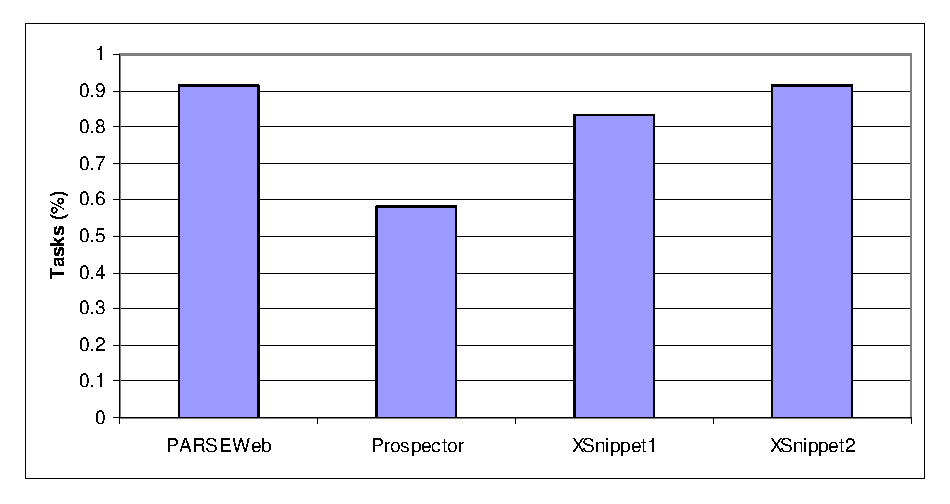
\includegraphics[scale=0.5,clip]{ComparisonResults.eps}\vspace*{-2ex}
\caption{Percentage of tasks successfully completed by PARSEWeb,
Prospector, and XSnippet} \label{fig:resultschart} \vspace*{-3ex}
\end{figure}
%-------------------------------------------------------------------------
\subsection{Summary}

The primary advantage of PARSEWeb compared to other related tools is
that PARSEWeb is not limited to the queries of any specific set of
frameworks or libraries. We showed this advantage in the first part
of our evaluation. Although Prospector solves the queries of a
specific set of frameworks or libraries from the API signatures, we
showed that the results of PARSEWeb are better than the results of
Prospector. The reason is that Prospector has no knowledge of which
MISs are often used compared to other
possible sets of sequences. This lack of information often results in
irrelevant solutions. Although both PARSEWeb and Strathcona suggest
solutions from code samples, the results of PARSEWeb are better than
Strathcona because the number of available code samples are limited
for Strathcona. Moreover, PARSEWeb has many specialized heuristics
compared to Strathcona for helping identify the required MIS. We
also showed that GCSE alone cannot handle the queries of the form
``\emph{Source} $\rightarrow$ \emph{Destination}'', and showed the
significance and impact of different techniques in PARSEWeb.
